\section{Аналитическая часть}

В данном разделе производится анализ предметной области. Даётся характеристика архитектурам современных ядрер операционных систем. Проводится краткий обзор ядра Linux, структур данных и его API. Описывается работа модуля ядра zram \cite{zram}, позволяющего хранить страницы виртуальной памяти в сжатом виде оперативной памяти.

\subsection{Постановка задачи}

Модуль ядра zram хранит оперативную память в сжатом в виде. При каждом обращении системы к участкам оперативной памяти, происходит преобразование данных: сжатие, при попытке записи данных в оперативную память, или возвращение к исходному (из сжатого) виду, при попытке чтения данных. Для проведения любого из этих преобразований центральному процессорному устройству необходимо затратить какое-то количество времени. При проведении сжатия, возможно вариант когда размер выходных (сжатых) данных не изменился или остался исходным \cite{data-compression}: процессорное время потрачено, а выигрыш в размере сжатых данных оказался минимален. Не всегда процент сжатия данных прямо пропорционален машинному времени, потраченному на эти преобразования \cite{data-compression}.

Таким образом, оптимизация метода сжатия страниц оперативной памяти должна определять (непосредственно до момента сжатия), соответствуют ли затраты процессорного времени, потраченные на сжатие данных, выигрышу в размере сжатых данных. Разработанный метод должен заранее определять, нужно ли сжимать страницу или хранить ее в несжатом виде.

\subsection{ЦПУ и оперативная память} 

Оперативная память (\cite{ram}) -- компонент, который позволяет компьютеру кратковременно хранить данные и осуществлять быстрый доступ к ним. Функции оперативной памяти реализуются с помощью специального технического устройства -- оперативного запоминающего устройства (ОЗУ). В этой памяти во время работы компьютера хранится выполняемый машинный код и данные, обрабатываемые центральным процессорным устройством (англ. central processing unit, CPU \cite{cpu}).

Проблему объема оперативной памяти компьютера можно решить увеличив количество планок ОЗУ. У данного подхода есть свои минусы:

\begin{itemize}
	\item электроэнергия -- каждая новая установленная планка увеличивает потребление энергии компьютера \cite{increasing-ram-bad};
	\item физические ограничения -- количество слотов для планок на материнской плате ограничено;
	\item стоимость -- каждая планка стоит денег.
\end{itemize}

Альтернативным решением является использование системы подкачки страниц (англ. paging \cite{paging}) -- специальный механизм операционный системы, при котором отдельные фрагменты памяти (мало используемые или полностью не активные) перемещаются из оперативной памяти во вторичное хранилище, например, на жёсткий диск или другой внешний накопитель. Несмотря на то что количество ОЗУ в таком случае увеличивается, доступ к таким участкам памяти замедляется -- системе приходится работать (читать и писать) с внешним запоминающим устройством, а такие устройства работают значительно медленнее ОЗУ \cite{ssd-hdd-speed}.

Ещё одним решением является сжатие данных прямо в оперативной памяти. Данный подход не имеет минусов выделенных у первого решения. Он реализуется программно и не требует закупки дополнительных планок ОЗУ. Кроме того, благодаря тому что сжатие не требует работы с внешним накопителем, скорость обработки данных увеличивается что позволяет избавиться от минуса (время работы) выделенного у второго решения. Сжатие данных так же имеет свои минусы, главным из которых является потребность в вычислительных ресурсах. ЦПУ должно выполнять инструкции для сжатия. Но, как и было отмечено во введении, чаще всего ЦПУ простаивает и не выполняет никакой работы, ожидая подсистему ввода/вывода.

\subsection{Сжатие данных}

Сжатие данных (англ. data compression \cite{data-compression-encyclopedia}) --  это способ (алгоритмический) преобразования информации в другую форму, чаще всего более компактную \cite{data-compression}. Сжатие основано на устранение избыточности, которая содержится в исходных данных. Примером является повторение в исходном тексте некоторых фрагментов. Такая избыточность устраняется заменой повторяющейся последовательности ссылкой на уже закодированный фрагмент с указанием его длины. Другой вид избыточности связан с тем, что некоторые значения в сжимаемых данных встречаются чаще других. Сокращение объёма данных достигается за счёт замены часто встречающихся данных короткими кодовыми словами, а редких -- длинными.

Все методы сжатия данных делятся на два класса: без потерь и с потерями. Сжатие данных без потерь позволяет полностью восстановить сжатые данные, в отличии от сжатия с потерями. Первый вариант чаще всего используют для сжатия текстовых данных и компьютерных программ, а сжатие с потерями используют для сокращения аудио- или видеоданных -- для таких данных не требуется полное соответствие исходным данным. Алгоритмы сжатия данных с потерями обладают большей эффективностью, чем алгоритмы без потерь \cite{lossless-compression}. В данной работе будут рассмотрены только алгоритмы сжатия данных без потерь: при работе с оперативной память терять данные непозволительно. На рисунке \ref{fig:conceptual-compressor} представлена концептуальная модель сжатия данных без потерь.

\begin{figure}[h]
	\centering
	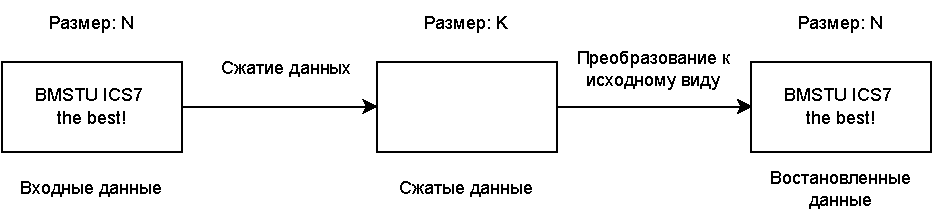
\includegraphics[width=\textwidth]{img/conceptual_compressor.pdf}
	\caption{Схема сжатия данных без потерь}
	\label{fig:conceptual-compressor}
\end{figure}

\subsubsection{Коэффициент сжатия}

Коэффициент сжатия -- характеристика алгоритмов сжатия данных, которая определяется формулой (\ref{fig:memory-compression}): 

\begin{equation}\label{fig:memory-compression}
	k = \frac{V_{original}}{V_{compressed}},
\end{equation}
где $V_{original}$ -- объём исходных данных, а $V_{compressed}$ -- сжатых.

Чем выше коэффициент сжатия, тем алгоритм эффективнее. При этом:

\begin{itemize}
	\item если $k = 1$, то алгоритм сжатия данных не производит. Сжатые данные по размеру равны исходным;
	\item если $k < 1$, то алгоритм сжатия данных создаёт еще больший (по размеру) блок данных, чем исходный.
\end{itemize}

\subsubsection{Требования к алгоритмам сжатия}

К алгоритмам сжатия могут применяться несколько требований:

\begin{itemize}
	\item скорость преобразования к сжатому виду;
	\item скорость преобразования к исходному виду;
	\item степень сжатия;
\end{itemize}

Для каждой конкретной задачи будут важны одни требования и менее важны другие. Так, например, для сжатия больших видеоданных с их последующим хранением, важнее будет степень сжатия данных, а не скорость работы алгоритма.

\subsection{Алгоритмы сжатия}

Главный принцип алгоритмов сжатия данных алгоритмов берет во внимание то, что в любом наборе (не случайном) данных, информация частично (либо,в редких случаях, полностью) повторяется \cite{lossless-compression}. С помощью математических методов можно определить вероятность повторения определенной комбинации байт. После этого можно создать создать некоторые коды, которые будут соответствовать наиболее распространяющимся наборам байт. Данные коды можно создать различными способами: энтропийное кодирование, кодирование повторов и сжатие с помощью словаря. С помощью указанных подходов возможно устранить дублирующую информацию из файла и уменьшить его итоговый размер (в сжатом виде). 

\subsubsection{Энтропийное кодирование}

Данный подход основывается на предположении о том, что до кодирования отдельные элементы последовательности данных имеют различную вероятность появления. После преобразований (кодирования) в результирующей последовательности вероятности появления отдельных элементов практически одинаковы \cite{lossless-compression}. Таким образом, энтропийное кодирование усредняет вероятности появления элементов в закодированное последовательности байт.

\subsubsection{Кодирование повторов} 

Кодирование повторов подразумевает замену повторяющихся символов (серии) на один символ и число его повторов. Серия -- последовательность данных, состоящих из одинаковых символов. Так, например, строка \\\texttt{a = IIIIIUUSEEVEEENNNNNNNN} может быть преобразована к виду \\\texttt{b = 5I2U1S2E1V3E8N}. В таком случае, коэффициент сжатия $k$ будет равен $k = \frac{len(a)}{len(b)} = \frac{22}{14} = 1.57$

Такое кодирование эффективно для наборов данных, содержащих большое количество серий -- например, простых графических изображений. 

\subsubsection{Сжатие с помощью словаря}

При использовании сжатия данных с помощью словаря данные делятся на слова, а сами слова в исходном наборе данных заменяются на их индексы в словаре. Чаще всего, словарь пополняется словами из исходной последовательности данных в процессе сжатия. 

Ключевым параметром такого метода сжатия является размер словаря. С одной стороны, чем больше его размер, тем больше эффективность сжатия. Однако, для неоднородного набора данных большой размер словаря может оказаться вреден. Например, при резком изменении типа данных большая часть словаря будет заполнена неактуальными словами. Кроме того, чем больше размер словаря, тем больше нужно дополнительной памяти для хранения слов в нём. 

Благодаря тому, что алгоритмическая сложность доступа к элементам словаря константа, алгоритмы сжатия с использованием словаря приводят данные к исходному виду быстрее, чем алгоритмы с использованием подходов, которые были описаны выше \cite{lossless-compression}.

\subsection{Информационная энтропия}

Информационная энтропия -- мера неупорядоченности или неопределенности состояния некоторой системы, описываемой данными. Вычисляется по формуле Шеннона (\ref{eq:shannon_entropy}):

\begin{equation}\label{eq:shannon_entropy}
	H(x) = -K\sum^n_{i=1}p(x_{i})log_2{p(x_{i})},
\end{equation}
где $p(x_{i})$ -- вероятность $i$-го состояния системы (значения принимаемого переменной), $n$ -- число состояний системы (значений, принимаемых переменной), $K$ -- положительная константа. Эта величина также называется средней энтропией сообщения. 

Величина, представленная на формуле \ref{eq:shannon_entropy_2}, называется частной энтропией и характеризует только $i$-e состояние системы.

\begin{equation}\label{eq:shannon_entropy_2}
	H(x) = -log_{2}{(p_{i})}.
\end{equation}

Функция \ref{eq:shannon_entropy} -- единственная функция, которая удовлетворяет ряду требований, необходимые для измерения энтропии:

\begin{enumerate}
	\item $H(p_{1},...,p_{n})$ определена и непрерывна для всех $p1,...,p_{n}$, где $p_{i} \in [0, 1]$ для всех $i=1,...,n$ и $p_{1}+...+p_{n} = 1$. Таким образом, функция зависит только от распределения вероятностей, но не от алфавита;
	\item для целых положительных $n$, должно выполняться неравенство \ref{eq:shannon_entropy_eq_1}:
	
	\begin{equation}\label{eq:shannon_entropy_eq_1}
		H(\frac{1}{n},...,\frac{1}{n}) < H(\frac{1}{n + 1},...,\frac{1}{n + 1});
	\end{equation}
	
	\item для целых положительных $b_{i}$, где $b_{1} + ... + b_{k} = n$, должно выполняться равенство \ref{eq:shannon_entropy_eq_2}:
	
	\begin{equation}\label{eq:shannon_entropy_eq_2}
		H(\frac{1}{n},...,\frac{1}{n}) = H(\frac{b_{1}}{n},...,\frac{b_{k}}{n}) + \sum^k_{i = 1}\frac{b_{i}}{n}H(\frac{1}{b_{i}},...,\frac{1}{b_{i}})
	\end{equation}
\end{enumerate}

Энтропия измеряется в битах, натах, тритах или хартли, в зависимости от основания логарифма, использующегося при вычислении энтропии. Логарифм используется в связи с тем, что он аддитивен для независимых источников. Так, например, энтропия события -- броска монеты, равна 1 биту (формула \ref{eq:moneta}), а энтропия $k$ бросков составит $k$ бит. 

\begin{equation}\label{eq:moneta}
	H(x) = -2(\frac{1}{2}log_{2}{\frac{1}{2}}) = -log_{2}{\frac{1}{2}}=log_{2}{2} = 1.
\end{equation}

В обычном представлении $log_{2}n$ бит требуется для представления переменной, принимающей $n$ значений, если $n$ является степенью 2. Если значения равновероятны, то энтропия в битах будет равна значению $n$.

\subsubsection{Бинарная энтропия}

Бинарная энтропия -- частный случай информационной энтропии, различие составляет лишь в том, что $x$ (формула \ref{eq:shannon_entropy_2}) может принимать только два значения: 0 или 1. Определяется как энтропия процесса Бернулли \cite{bernoulli-process} с вероятностью $p$ одного одного из двух значений. Рассчитывается по формуле Хартли (\ref{eq:binary_entropy}):

\begin{equation}\label{eq:binary_entropy}
	i = log_{2}{N},
\end{equation}
где $N$ -- мощность алфавита, $i$ -- количество информации в каждом символе сообщения. Для случайно величины $x$, принимающей $n$ независимых случайных значений $x_{i}$ с вероятностями $p_{i}(i = 1,...,n)$ формула Хартли переходи в формулу Шеннона (\ref{eq:shannon_entropy}).

На рисунке \ref{fig:binary_entropy} представлена функция бинарной энтропии.

\begin{figure}[h]
	\centering
	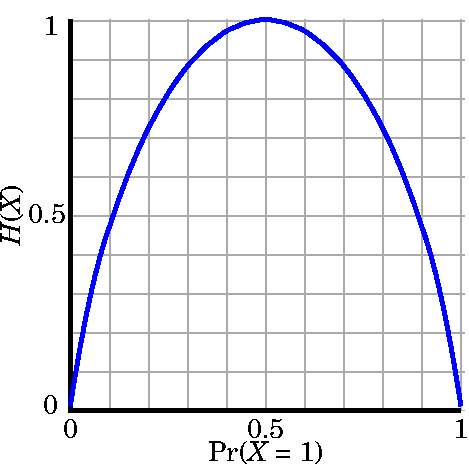
\includegraphics[scale=1]{img/entropy.pdf}
	\caption{Функция бинарной энтропии}
	\label{fig:binary_entropy}
\end{figure}

\subsubsection{Энтропия и сжатие данных}

Энтропия набора данных является мерой количества содержащейся в нем информации \cite{entropy-paper}. Информационная энтропия, подсчитанная для данных, размер которых известен, можно использовать чтобы получить теоретическую границу того, насколько эти данные могут быть сжаты \cite{entropy-paper}. Таким образом, рассчитав энтропию для некоторых данных, можно предсказать их примерный размер после проведения преобразования сжатия.

Для вычисления энтропии набора данных, в среднем, требуется в несколько раз меньше машинного времени, чем для сжатия этого набора данных \cite{entropy-paper}. Этот факт можно использовать для ускорения процесса сжатия, если алгоритм сжатия вызывается повторно. Например если данные, которые нужно сжать, разбиты на участки, что может быть актуально при параллельной обработке данных. Можно считать энтропию для каждого такого участка, и на основе полученного значения принимать решение, сжимать этот участок или хранить в несжатом виде. В таком случае, время сжатия увеличиться, но при этом итоговый коэффициент сжатия данных будет уменьшен. Можно сделать вывод, что чем больше таких участков и чем больше энтропия сжимаемых участков, тем больше будет выигрыш во времени и меньше проигрыш в сжатии данных.

\subsection{Ядра операционных систем}

Ядро операционной системы -- это программное обеспечение, которое предоставляет базовый функционал для всех остальных частей операционной системы, управляет аппаратным обеспечением и распределяет системные ресурсы \cite{kernel-development}. Ядра операционных систем можно разделить на две группы: с монолитным или с микроядром.

Монолитное ядро является самым простым, оно реализовано в виде одного большого процесса, который выполняется в одном адресном пространстве. Все службы ядра находятся и выполняются в одном адресном пространстве. Благодаря этому, взаимодействия в ядре осуществляются очень просто, так, например, ядро может вызывать функции непосредственно, как это делают пользовательские приложения \cite{kernel-development}. Из-за отсутствия издержек, таких как синхронизация процессов и передача данных между ними, монолитные ядра операционных систем являются более производительным, чем микроядра. На рисунке \ref{fig:monolithic kernel} представлена концептуальная модель операционной системы с монолитном ядром.

\begin{figure}[h]
	\centering
	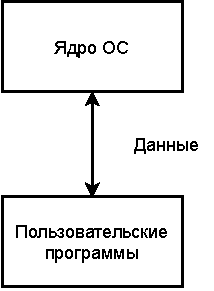
\includegraphics[scale=2]{img/monolithic_kernel.pdf}
	\caption{Схема ОС с монолитным ядром}
	\label{fig:monolithic kernel}
\end{figure}
 
Реализация микроядра подразумевает отказ от одного большого процесса. Все функции ядра разделяются на несколько процессов, которые обычно называют серверами \cite{kernel-development}. При этом, в привилегированном режиме могут работать лишь те сервера (процессы), которым этот режим необходим, а остальные сервера работают в непривилегированном (пользовательском) режиме. К первым типам процессов можно отнести, например, механизмы управления памятью компьютера, а ко вторым драйвера устройств. При таком подходе все сервера изолированы и работают в независящем друг от друга адресном пространстве, то есть прямой вызов функций (как в монолитном ядре) невозможен. Все взаимодействия между серверами происходит с помощью механизма межпроцессного взаимодействия (англ. Interprocess Communcation, IPC \cite{ipc}), а обеспечивает передачу данных само ядро (больше никаких действий в системе оно не выполняет). Такой подход позволяет предотвратить возможность выхода из строя одного сервера при выходе из строя другого и позволяет по по мере необходимости одному серверу выгрузить из памяти другой. Но, как уже было отмечено выше, такая модель имеет более низкую производительность из-за накладных расходов на IPC. На рисунке \ref{fig:micro_kernel} представлена концептуальная схема операционной системы с монолитном ядром. 

\begin{figure}[h]
	\centering
	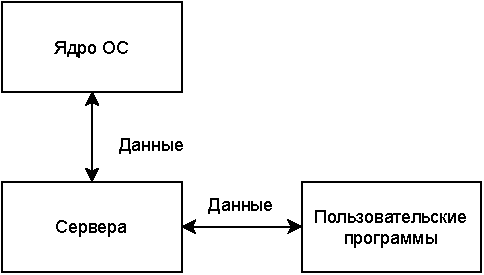
\includegraphics[width=\textwidth]{img/micro_kernel.pdf}
	\caption{Схема ОС с микроядром}
	\label{fig:micro_kernel}
\end{figure}

\subsection{Ядро Linux}

Ядро Linux \cite{linux} -- ядро операционной системы с открытым исходным кодом, распространяющееся как свободное программное обеспечение. Именно из-за этого в данной работе будет рассмотрено данное ядро. Ядро Linux является монолитным. Но, несмотря на это, при разработке ядра была из микроядерной модели были позаимствованы некоторые решения: модульный принцип построения, приоритетное планирование самого себя, поддержка многопоточного режима и динамической загрузки в ядро внешних бинарных файлов (модулей ядра) \cite{kernel-development}. Linux не использует никаких функций микроядерной модели (IPC), которые приводят к снижению производительности системы.

Ниже представлены отличительные черты ядра Linux:

\begin{itemize}
	\item потоки ничем не отличаются от обычных процессов. С точки зрения ядра все процессы одинаковы и лишь некоторые из них делят ресурсы между собой;
	\item динамическая загрузка модулей ядра;
	\item приоритетное планирование. Ядро способно прервать выполнение текущего процесса, даже если оно выполняется в режиме ядра;
	\item объектно-ориентированная модель устройств. Ядро поддерживает классы устройств и события;
	\item ядро Linux является результатом свободной и открытой модели разработки \cite{kernel-development}.
\end{itemize}

\subsubsection{Основные компоненты ядра}

Ядро Linux состоит из нескольких основных компонентов:

\begin{itemize}
	\item планировщик процессов -- определяет, какой из процессов должен выполняться, в какой момент и как долго;
	\item менеджер памяти -- обеспечивает работу виртуальной памяти и непосредственно доступ к ней;
	\item виртуальная файловая система -- специальный единый файловый интерфейс, скрывающий интерфейс физических устройств;
	\item сетевые интерфейсы -- обеспечивают работу с сетевым оборудованием;
	\item межпроцессная подсистема -- механизмы межпроцессного взаимодействия.
\end{itemize}

\subsubsection{Страничная организация памяти}

Работа с памятью в ядре Linux организована с помощью примитива страниц. Страница памяти -- набор некоторого количества байт. Хотя наименьшими адресуемыми единицами памяти являются байт и машинное слово, такой подход не является удобным \cite{kernel-development}. Размер страницы это фиксированная константа \texttt{PAGE\_SIZE}, которая на большинстве современных архитектур, поддерживаемых Linux, составляет 4 Кб \cite{4kb-page-size}. Страничная организация памяти позволяет реализовать внутри ядра Linux механизм виртуальной памяти.

\subsubsection{Виртуальная память}

Виртуальная память -- специальный механизм организации памяти, при котором процессы работают не с физическими адресами напрямую, а с виртуальными. С помощью такого подхода в ядре Linux реализуется защита адресного пространства процессов, так, например, процесс не может получить доступ к памяти другого процесса и внести туда изменения.

В ядре каждая физическая страница памяти описывается с помощью структуры \texttt{struct page}. Рассматриваемая структура с наиболее важными полями представлена в листинге \ref{code:struct_page}.

\newpage

\begin{code}
	\captionof{listing}{Структура \texttt{struct page}}
	\label{code:struct_page}
	\inputminted
	[
	frame=single,
	framerule=0.5pt,
	framesep=20pt,
	fontsize=\small,
	tabsize=4,
	linenos,
	numbersep=5pt,
	xleftmargin=10pt,
	]
	{text}
	{code/struct_page.c}
\end{code}

Ниже представлено описание наиболее важных полей данной структуры:

\begin{itemize}
	\item \texttt{flags} -- флаги, которые хранят информацию о состоянии страницы в текущий момент, например, находится ли данная страница в кэше или нет. Каждый флаг представляет из себя один бит;
	\item \texttt{\_refcount} -- счётчик ссылок на страницу. Если значение этого счётчика равно -1, это означает что страница нигде не используется;
	\item \texttt{virtual} -- виртуальный адрес страницы, соответствует адресу страницы в виртуальной памяти ядра;
	\item \texttt{\_last\_cpupid} -- номер последнего ЦПУ, использовавшего данную страницу.
\end{itemize}

Рассматриваемая структура данных в ядре используется для учёта всей физической памяти.

В ядре Linux предусмотрен специальный низкоуровневый механизм для выделения памяти и несколько интерфейсов доступа к ней. Прототип функции основной функции выделения памяти представлен в листинге \ref{code:alloc_pages}.

\begin{code}
	\captionof{listing}{Прототип функции \texttt{alloc\_pages}}
	\label{code:alloc_pages}
	\inputminted
	[
	frame=single,
	framerule=0.5pt,
	framesep=20pt,
	fontsize=\small,
	tabsize=4,
	linenos,
	numbersep=5pt,
	xleftmargin=10pt,
	]
	{text}
	{code/alloc_pages.c}
\end{code}

С помощью функции \texttt{alloc\_pages} можно выделить $2^{order}$ смежных страниц физической памяти. Функция возвращает указатель на структуру \texttt{struct page}, которая соответствует первой выделенной странице памяти. Для выделения одной страницы памяти используется функция \texttt{alloc\_page} (листинг \ref{code:alloc_page}).

\begin{code}
	\captionof{listing}{Прототип функции \texttt{alloc\_page}}
	\label{code:alloc_page}
	\inputminted
	[
	frame=single,
	framerule=0.5pt,
	framesep=20pt,
	fontsize=\small,
	tabsize=4,
	linenos,
	numbersep=5pt,
	xleftmargin=10pt,
	]
	{text}
	{code/alloc_page.c}
\end{code}

На рисунке \ref{fig:memory_schema} представлена схема управления страницами памяти в ядре Linux.

\begin{figure}[h]
	\centering
	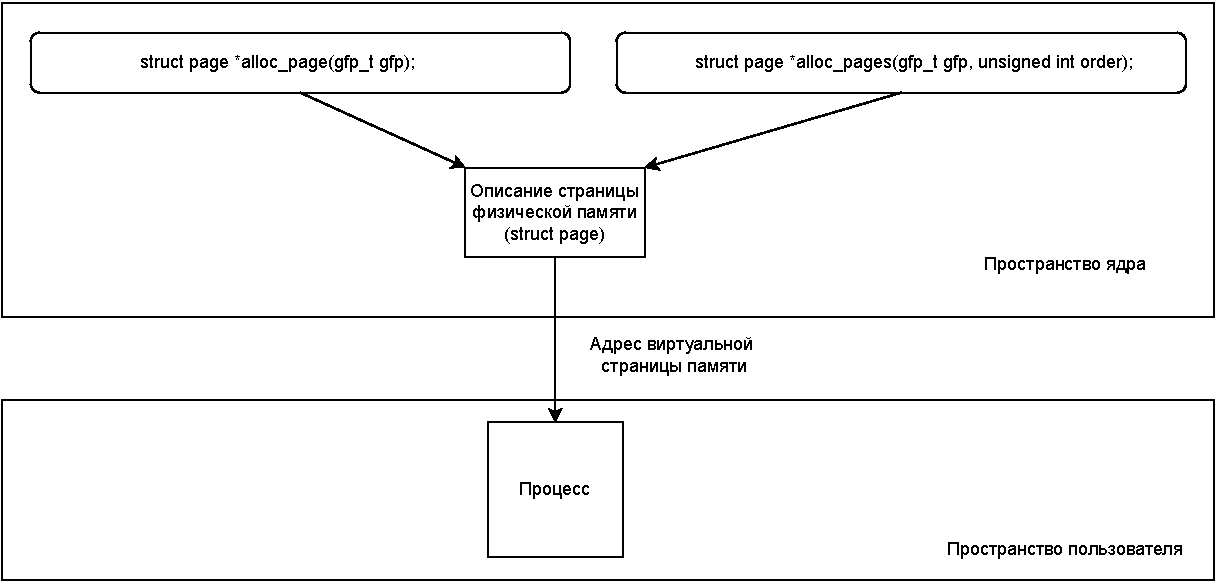
\includegraphics[width=\textwidth]{img/memory.pdf}
	\caption{Схема управления памятью}
	\label{fig:memory_schema}
\end{figure}

\subsubsection{Подкачка страниц}

Подкачка страниц -- специальный механизм внутри ядра Linux, который реализован благодаря механизму виртуальной памяти, при котором отдельные страницы оперативной памяти записываются не в ОЗУ, а, чаще всего, в специальное вторичное хранилище, например, жесткий диск. Ядро само выбирает, какие страницы памяти попадут в это хранилище. Чаще всего, это неактивные или реже всего использующиеся страницы памяти. 

Выгруженные из оперативной памяти страницы могут храниться как в специальном разделе жесткого диска, так и в файле. Пространство, где хранятся эти страницы, называется swap-пространством. При попытке обратиться к выгруженной странице, в ядре происходит исключительная ситуация, называемая page fault \cite{page-fault}. Обработчик прерываний обрабатывает данный запрос и перемещает страницу обратно в оперативную память. На рисунке \ref{fig:swap} представлена схема работы подсистемы подкачки страниц в ядре Linux.

\begin{figure}[h]
	\centering
	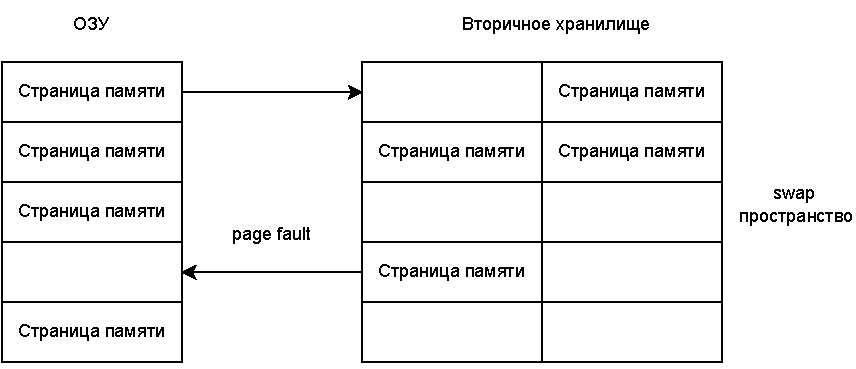
\includegraphics[width=\textwidth]{img/swap.pdf}
	\caption{Подсистема подкачки страниц}
	\label{fig:swap}
\end{figure}

\subsubsection{Блочные устройства}

Блочное устройство -- специальный интерфейс в ядре Linux, обеспечивающий доступ к реальному или виртуальному устройству \cite{block-devices}. Представляет из себя файл в файловой системе. Блочные устройства характеризуются случайным доступом к данным, организованным в блоки фиксированного размера. Примерами таких устройств являются жестки диски, приводы CD-ROM, RAM-диски и т.д. Скорость блочных устройств, как правило, намного выше, чем скорость символьных устройств \cite{character-devices}. В символьных устройствах данные обрабатываются последовательно, без возможности произвольного доступа и по одному символу. Ядро Linux предоставляет специальное API для работы с блочными устройствами.

Работать с блочными устройствами сложнее, чем с символьными. Символьные устройства имеют одну текущую позицию, в то время как блочные устройства должны иметь возможность перемещаться на любую позицию в устройстве, для того чтобы обеспечить произвольный доступ к данным. Для упрощения работы с блочными устройствами ядро Linux представляет подсистему называемую подсистемой блочного ввода-вывода.

С точки зрения ядра наименьшей логической единицей адресацией является блок. Хотя физическое устройство может быть адресовано на уровне сектора, ядро выполняет все дисковые операции с использованием блоков. Поскольку наименьшей единицей физической адресации является сектор, размер блока должен быть кратен размеру сектора. Кроме того, размер блока должен выполнять требование \ref{eq:nepridymalnazvanie} (размер должен быть кратен цифре два, возведенную в любую степень) и не может превышать размер страницы памяти (PAGE\_SIZE). 

\begin{equation}\label{eq:nepridymalnazvanie}
	block\_size \; mod \; 2^N = 0, N \in [0, \inf]
\end{equation}

Размер блока может варьироваться в зависимости от используемой файловой системы, наиболее распространенными значениями являются 512 байт, 1 килобайт или 4 килобайта \cite{block-devices}.

На рисунке \ref{fig:block-devices} представлена схема взаимодействия блочного и физического устройства.

\begin{figure}[h]
	\centering
	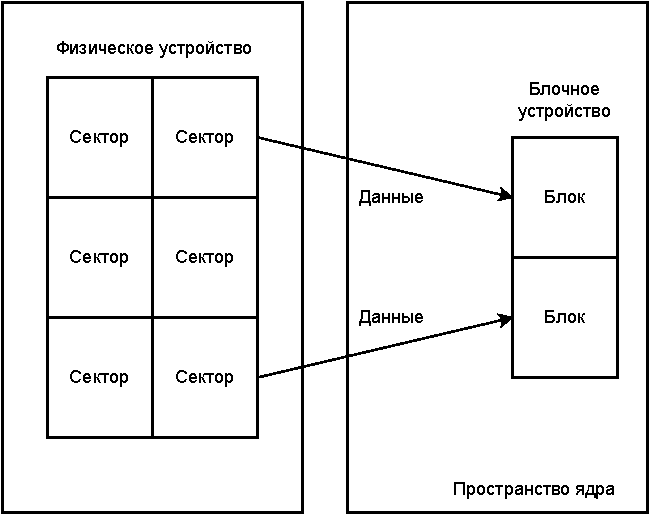
\includegraphics[width=\textwidth]{img/block-devices.pdf}
	\caption{Схема взаимодействия блочного и физического устройства}
	\label{fig:block-devices}
\end{figure}

\subsection{Модуль ядра zram}

Модуль ядра zram создает в оперативной памяти специальное блочное устройство. Такое устройство можно создать из пространства пользователя. Страницы памяти, попадающие в это устройство, сжимаются и хранятся прямо в оперативной памяти. Такой подход обеспечивает экономию памяти и быстрый ввод/вывод, по сравнению с использованием дисковых хранилищ \cite{zram}. 

Созданное блочное устройство zram можно установить в качестве системы подкачки (swap) или в качестве в блочного устройства для файловых хранилищ, хранящихся в оперативной памяти. Примером такого хранилища  является tmpfs \cite{tmpfs}. 

Но, чаще всего, zram используется в паре с swap. Механизм swap отправляет страницу в zram через подсистему блочного ввода-вывода. Сжатая страница внутри zram идентифицируется уникальным ключом $zkey$ (\ref{fig:zkey}):

\begin{equation}\label{fig:zkey}
	zkey = device\_id + offset
\end{equation}
где $device\_id$ -- идентификатор устройства подкачки, а $offset$ -- смещение страницы.

Когда система подкачки определяет, что какая-либо из страниц, хранящихся в устройстве подачки, необходима пользователю (когда происходит прерывание page fault), устройство zram уведомляется, о том, что необходимо привести запрашиваемую страницу с идентификатор $zkey$ преобразовать к исходному виду и вернуть её системе. Пока данные находятся в сжатом состоянии, система не может прочитать или записать какие-либо отдельные байты из этой сжатой последовательности. Современные алгоритмы могут сжимать любое количество последовательных байт. Несмотря на это, модуль ядра zram использует работает лишь с виртуальными страницами памяти.

Для достижения высокой степени сжатия требуется выполнение большого количества команд ЦПУ, тогда как менее эффективное сжатие может выполняться быстрее. В ядре необходимо добиться баланса между временем и степенью сжатия. Кроме того, важно чтобы выбор алгоритма оставался гибким. Например для выполнения одной задачи подойдёт один алгоритм сжатия, а для второй другой. В модуле ядре zram существует специальное API, доступное из пространства пользователя, для выбора алгоритма сжатия. Данный модуль поддерживает несколько алгоритмов сжатия, например DEFLATE \cite{deflate}, LZ4 \cite{lz4}, LZO \cite{lzo}, LZO-RLE\cite{lzo-rle} 842 \cite{842}, zstd \cite{zstd}. 

Из-за того что размер страницы достаточно большой (4 Кб), сжатие и восстановление данных -- дорогостоящие операции, поэтому необходимо ограничить количество этих операций. Нужно тщательно выбирать, какие страницы стоит сжимать, а какие нет. Алгоритм, реализованный в ядре Linux, определяющий какие страницы нужно сжимать, выбирает те страницы, которые вероятно будут использоваться снова, но вряд ли будут использоваться в ближайшем будущем \cite{in-kernel-memory-compression}. Такая реализация позволяет не тратить всё время ЦПУ на многократное сжатие и распаковку страниц. Кроме того, необходимо чтобы ядро могло идентифицировать сжатую страницу -- иначе её невозможно найти и распаковать.

Размер страницы, к которой был применён алгоритм сжатия зависит от данных на исходной странице. Степень сжатия страницы описывается следующей формулой (\ref{fig:page-compressing}):

\begin{equation}\label{fig:page-compressing}
	k = \frac{PAGE\_SIZE}{zsize},
\end{equation}
где \texttt{PAGE\_SIZE} размер страницы памяти в системе, а \texttt{zsize} -- размер сжатой страницы. 

Чаще всего, размер сжатой страницы меньше чем \texttt{PAGE\_SIZE}, поэтому, обычно, коэффициент сжатия меньше единицы. Но, в некоторых случаях, коэффициент сжатия может быть больше единицы. В среднем страница памяти в ядре сжимается в два раза \cite{in-kernel-memory-compression}, то есть коэффициент сжатия $ k =\frac{1}{2}$.

Неудачная попытка записать блок в подсистему блочного вывода приводит к большим накладным расходам \cite{in-kernel-memory-compression}. По этой причине, при сохранении страницы памяти со степенью сжатия $k < 1$, zram сохраняет исходную страницу памяти (не сжатую) в ОЗУ, что в конечном итоге не приводит к экономии места.

В ядре модуль описывается с помощью структуры \texttt{struct zram} (листинг \ref{code:zram}).
\begin{code}
	\captionof{listing}{Структура \texttt{struct zram}}
	\label{code:zram}
	\inputminted
	[
	frame=single,
	framerule=0.5pt,
	framesep=20pt,
	fontsize=\small,
	tabsize=4,
	linenos,
	numbersep=5pt,
	xleftmargin=10pt,
	]
	{text}
	{code/zram.c}
\end{code}

Данная структура хранит в себе массив сжатых страниц, семафор, с помощью которого достигается синхронизация при параллельной обработке \cite{in-kernel-memory-compression}, название алгоритма, который будет производить сжатие, размер блочного устройства, статистику по проведенным операциям и другие поля.

Для хранения информации о сжатых страницах (их размер и данные) используется массив структур. Это необходимо, для того чтобы найти эту страницу для её дальнейшего преобразования к исходному (не сжатому) виду. Элементом массива является структура \texttt{struct zram\_table\_entry}, которая представлена в листинге \ref{code:zram_table_entry}.

\begin{code}
	\captionof{listing}{Структура \texttt{struct zram\_table\_entry}}
	\label{code:zram_table_entry}
	\inputminted
	[
	frame=single,
	framerule=0.5pt,
	framesep=20pt,
	fontsize=\small,
	tabsize=4,
	linenos,
	numbersep=5pt,
	xleftmargin=10pt,
	]
	{text}
	{code/zram_table_entry.c}
\end{code}

Для идентификации страниц и управления данными данный модуль использует прямой поиск по таблице страниц (массив из структур \\\texttt{struct zram\_table\_entry}), которая хранится в структуре \texttt{struct zram}.

Для корректной параллельной обработки страниц используется семафор \\\texttt{struct rw\_semaphore}.

zram устраняет дубликаты страниц, которые состоят из одного и того же элемента. В таком случае, сохраняется лишь один этот элемент. Несмотря на то, чтобы определить, состоит ли страница полностью из одинаковых байт, требуются накладные расходы, эти расходы чаще всего небольшие, по сравнению с затратами на сжатие \cite{in-kernel-memory-compression}.

На рисунке \ref{fig:zram-kernel} представлена модель взаимодействия модуля zram, ядра и пользователя.

\begin{figure}[h]
	\centering
	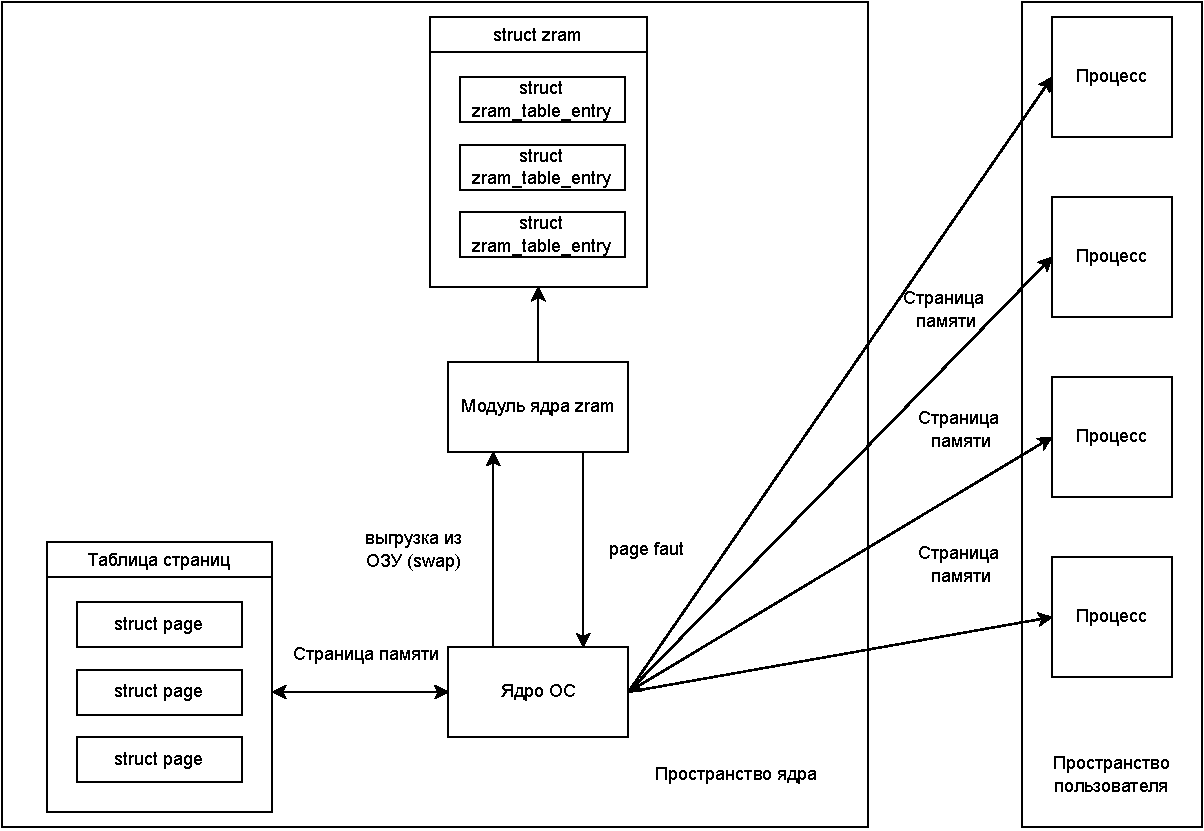
\includegraphics[width=\textwidth]{img/zram-kernel.pdf}
	\caption{Модель взаимодействия zram, ядра и пользователя}
	\label{fig:zram-kernel}
\end{figure}

\subsubsection{Опция writeback}

Модуль ядра zram предоставляет возможно опционально включить специальную опцию writeback, которая позволяет сохранять неиспользуемые или несжимаемые страницы во вторичное хранилище, а не в оперативную память. Для реализации данного функционала структура \texttt{struct zram} хранит в себе указатель на структуру \texttt{struct block\_device} (см. листинг \ref{code:zram}). Структура \texttt{struct block\_device} представлена на листинге \ref{code:struct_block_device}.

Данная структура является описанием некоторого блочного устройства внутри ядра Linux. В случае модуля zram, структура \texttt{struct block\_device} описывает вторичное хранилище, в которое будут отправляться несжимаемые или неиспользуемые страницы оперативной памяти при включенной опции\\ writeback.

\begin{code}
	\captionof{listing}{Структура \texttt{struct block\_device}}
	\label{code:struct_block_device}
	\inputminted
	[
	frame=single,
	framerule=0.5pt,
	framesep=20pt,
	fontsize=\small,
	tabsize=4,
	linenos,
	numbersep=5pt,
	xleftmargin=10pt,
	]
	{text}
	{code/struct_block_device.c}
\end{code}

\subsection{Вывод}

В данном разделе был проведен анализ предметной области: были рассмотрены понятия сжатия данных, оперативной памяти и информационной энтропии. Была дана характеристика алгоритмам сжатия. 

Были характеризованы современные ядра операционных систем: с монолитной и микроядерной архитектурой. Проведён краткий обзор ядра Linux, структур данных и API управления подсистемой памяти внутри ядра. 

Была описана работа модуля ядра zram, позволяющего хранить страницы виртуальной памяти в сжатом виде оперативной памяти: приведен обзор используемых структур и схему взаимодействия zram, ядра и пользователя.

\pagebreak
